\section{The CAIP Dataset}
\label{sec:data}

This paper introduces the CraftAssist Instruction Parsing (CAIP) dataset of English-language commands and their associated logical forms (see Appendix~\ref{sec:dataset_examples} for examples and Appendix \ref{sec:action_tree} for a full grammar specification).  
\begin{comment}
The  number of examples of each kind as well as the training/test split are presented in Table~\ref{tab:dataset_stats}.

\begin{table}[t!]
\center
\begin{tabular}{l|ccc}
Split       & Train   	& Val    & Test \\
\midrule % & Total  \\ \hline
%Templated   & 510K  	& 5K     & 5K   \\ % & 4     \\
%Rephrases   & 27K     	& 2K     & 2370  \\ % & 8     \\
Prompts     & -       	& 1500   & 3032 \\ %  & 12    \\
Interactive & -       	& 661    & 1500  \\ %  & 16    \\ \hline
\end{tabular}
\caption{Data splits for all data collection processes. \label{tab:dataset_stats}}
\end{table}



\subsection{Templated Data}
\label{sec:generated_data}

We algorithmically generate logical forms over the grammar with associated surface forms through the use of templates. To that end, we first define a set of {\it template objects}.  These might  link a concept in the game world to several ways it can be described through language.  For example the template object \texttt{Move} links the action type \textsc{move} to the utterances \textit{go},  \textit{walk},  \textit{move},\ldots 
%Likewise, the template object \texttt{RelativeDirection} links all of the assistant's direction primitives to their names. 
 Other template objects have purely decorative functions (w.r.t. the assistant's action space), for example \texttt{Please}.
 %and are in order to make the sentence more natural. For example, the object \texttt{ALittle} can be realized into \textit{a bit},  \textit{a little}, \textit{somewhat}, \ldots . 
 The set of possible realizations for each template object is manually defined.

Then, we build {\it templates} for each action as recursive sequences of templates and template objects. For each of these templates, we can then sample a game value and its corresponding string. By concatenating these, we obtain a logical form and its corresponding language description. Consider for example the template [\texttt{Move}, \texttt{ALittle}, \texttt{RelativeDirection}].% made up of the template objects described above. 
One possible realization could be the description \textit{go a little to the left} paired with a logical form specifying the action type as \textsc{move}, and an \textsc{action location} sub-tree with which a child relative direction categorical node which has value \textsc{left}. 

%We handle compositionality by combining different action templates together in order, for example to generate: \textit{go there and build me a big circle}  we combined respective templates from \textsc{move} action and \textsc{build} action to give an ordered sequence of actions under ``action\_sequence'' in the tree. 

We generate
training data for the \textsc{noop} action type by sampling dialogue lines from the Cornell Movie Dataset \cite{Danescu-Niculescu-Mizil+Lee:11a}.


We wrote 3,900 templates in total. We can create a training example for a parsing model by choosing a template at random, and then sampling a (description, tree) pair from it, which, given the variety and modularity of the template objects, yields virtually unlimited data (for practical reasons, we pre-generate a set of 510K training, 5K validation, and 5K test examples for our experiments). The full list of templates and template objects is included in the Supplementary Material.

% We generated a large database of natural language commands and their corresponding action trees using a system of hierarchically composable templates. Each action is characterized by a set of supported templates, each of which is an ordered list of template objects.

% To generate a command, we choose a random action from the set of supported actions (a complete list is presented in section \ref{sec:action_tree}) and then a random template is chosen from the action's template set. Each template object is then converted to text to produce the command, and key-value pairs to produce the action tree.

% An example template for the \textsc{Move} action is composed of the  objects. Given different resolutions of each object, the template might produce commands like "move a little to the right" or "can you walk a bit south". Some template objects affect the action tree (e.g. the "relative\_direction" key is different in the two examples above), while others like \texttt{ALittle} do not.

% Template objects may also make use of other template objects, making the conversion to text a recursive process. The text and action tree fragments produced by template objects that are shared across templates can be reused (e.g. both the \textsc{Move} and \textsc{Build} actions may specify a \texttt{Location}).

\end{comment}




\begin{figure}
\center
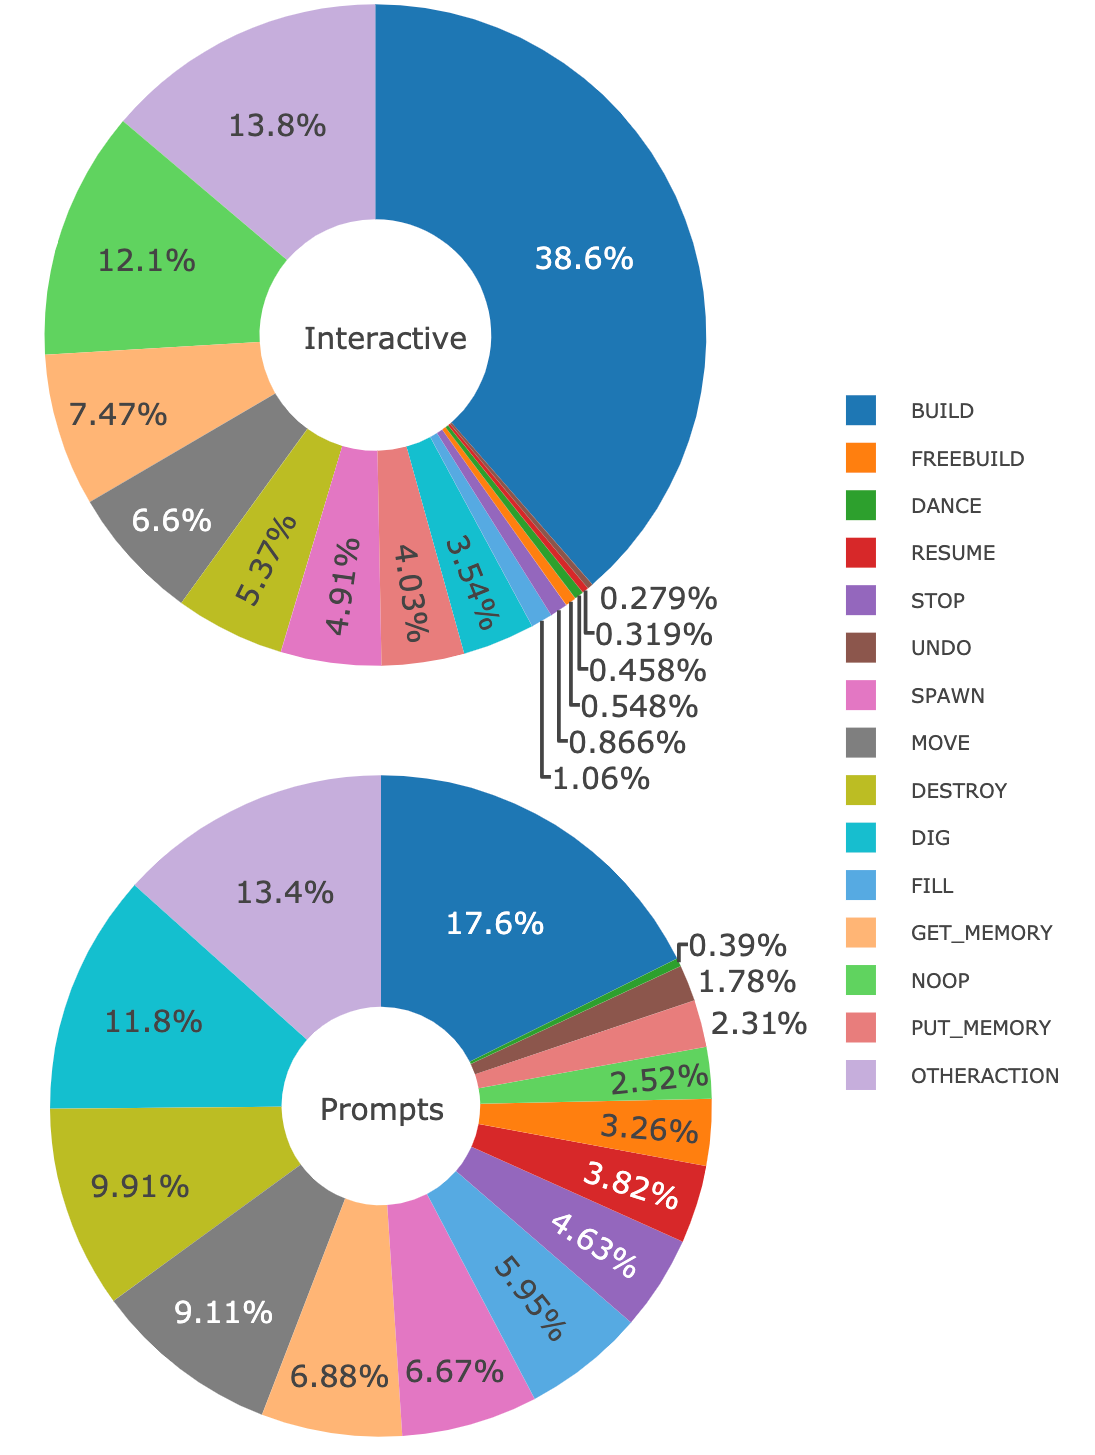
\includegraphics[width=0.9\linewidth ]{figures/action_freq2_vert.png}
\caption{Frequency of each action type in the different data collection schemes described in Section~\ref{sec:collected_data}.
\label{fig:action_freqs}
}
\end{figure}

\subsection{Collected Data}
\label{sec:collected_data}

%To supplement the generated data, 
We collected natural language commands written by crowd-sourced workers  in a variety of settings. The complete list of instructions given to crowd-workers in different settings, as well as step-by-step screen-shot of the annotation tool, are provided in the Appendix \ref{sec:instructions}.  The basic data cleanup is described in Appendix \ref{sec:data_cleanup}.

\begin{figure}
\center
%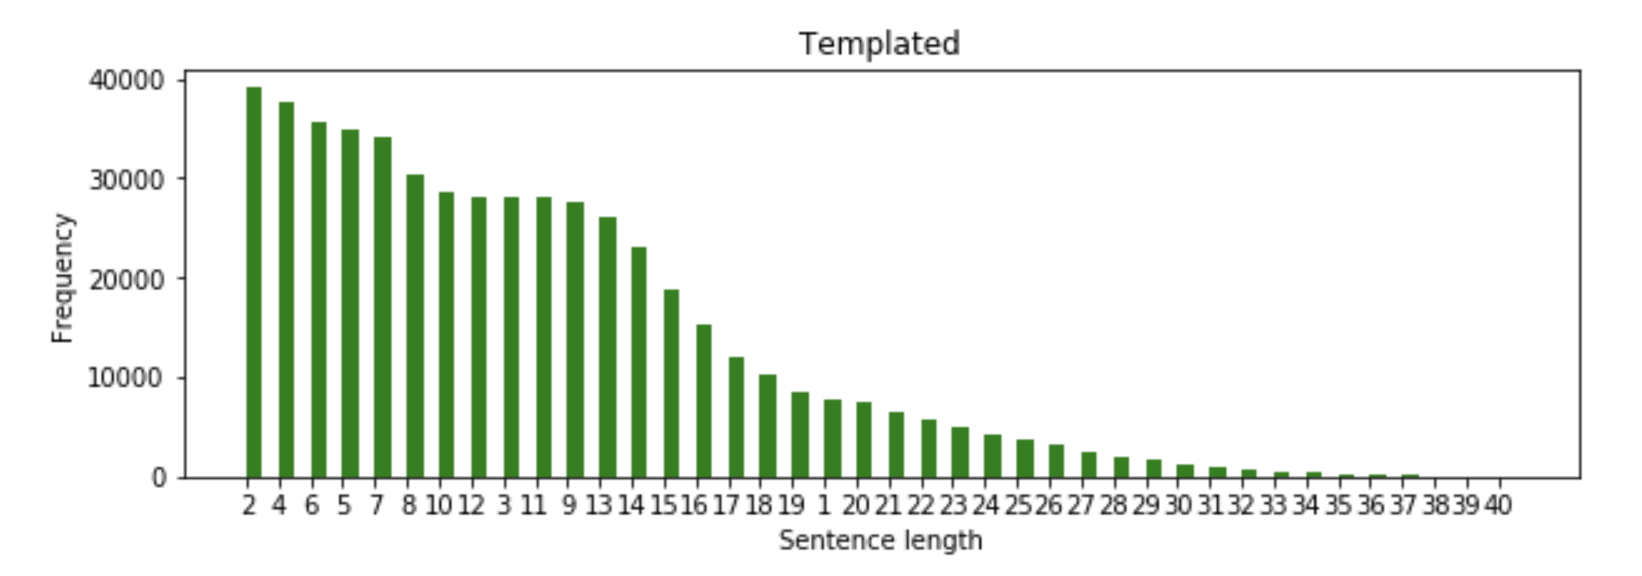
\includegraphics[width=0.3\linewidth ]{figures/sent_len_temp.png}
\hspace*{-.2cm}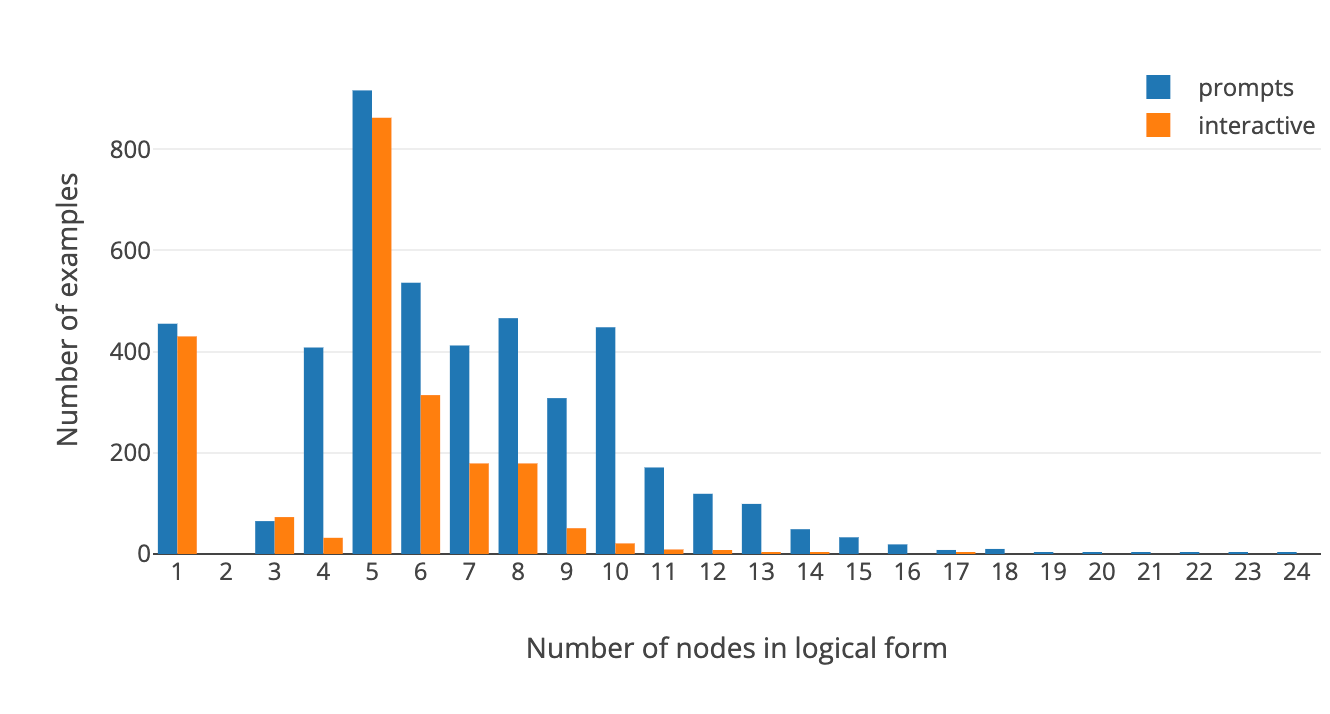
\includegraphics[width=1\linewidth, height=0.35\linewidth]{figures/nodenum_histogram}
\hspace*{-.2cm}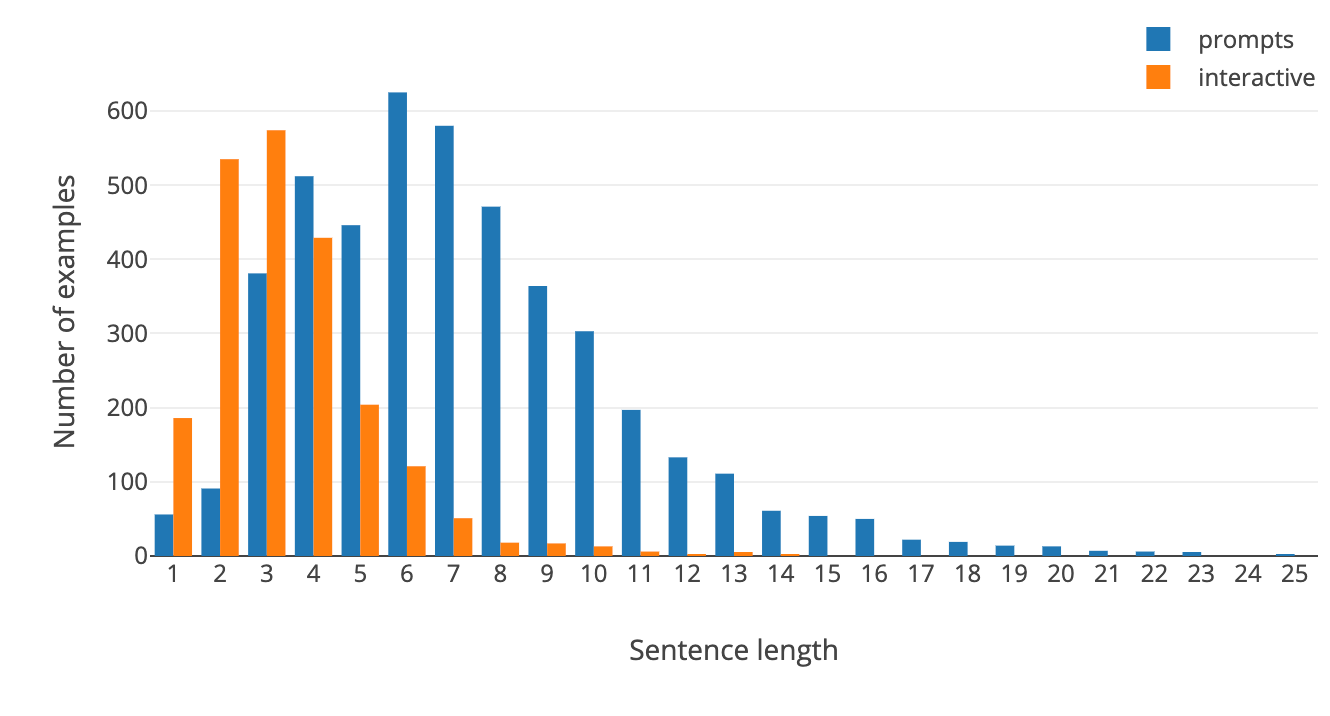
\includegraphics[width=1\linewidth, height=0.35\linewidth]{figures/sentence_length_histogram}
\caption{Histograms showing distribution over number of nodes in a logical form (top) and utterance length in words (bottom) for each data type. Prompts averages 6.74 nodes per logical form, 7.32 words per utterance, and interactive averages 4.89, 3.42 respectively}
\label{fig:quant_sent_len}
\end{figure}



%\subsubsection{Rephrases} While the template generations yield a great variety of language, they cannot cover all possible ways of phrasing a specific instruction. In order to supplement them, we asked crowd-sourced workers to  rephrase some of the produced instructions into commands in alternate, natural English that does not change the meaning of the sentence. This setup enables the collection of unique English commands whose action trees are already known. Note that a rephrased sentence will have the same action tree structure, but the positions of the words corresponding to span nodes may change. % , and hence the values of the spans.
% For example, the command "build a pillar", represented by the action tree:  \{"Build": \{"schematic": \{"has\_name\_": [2,~2]\}\}\}, might be rephrased to "make me a pillar", where the word "pillar" has now moved to index 3. 
%To account for this, words contained in a span range in the original sentence are highlighted in the task, and crowd-sourced workers are asked to highlight the corresponding words in their rephrased sentence. Then the action tree span values are substituted for the rephrased sentence to get the corresponding tree. This yields a total of 32K rephrases.
%We selected the instructions to be rephrased at random and assessed the quality of rephrases by throwing away all mistakes made by humans when highlighting the spans. If the any spans were missing or the highlighting wasn't done properly, we threw the rephrase data away.
% We use 30K for training, 1K for validation, and 1K for testing.


\subsubsection{Image and Text Prompts} \label{sec:prompts}We presented crowd-sourced workers with a description of the capabilities of an assistant bot in a creative virtual environment (which matches the set of allowed actions in the grammar), and (optionally) some images of a bot in a game environment. They were then asked to provide examples of commands that they might issue to an in-game assistant. We refer to these instructions as ``prompts'' in the rest of this paper.
% The complete instructions shown to workers is included in appendix \ref{fig:freegen}.

% The process of annotating these sentences with their corresponding action trees is described in section \ref{sec:annotation_tool}.

\subsubsection{Interactive Gameplay}\label{sec:human_bot} We asked crowd-workers to play creative-mode Minecraft with our assistant bot, and they were instructed to use the in-game chat to direct the bot as they chose. The game sessions were capped at 10 minutes and players in this setting had no prior knowledge of the bot's capabilities or the grammar. We refer to these instructions as ``Interactive'' in the rest of this paper.
The instructions of this setting are included in Appendix \ref{sec:appen}. 
% Each line of in-game chat written by a player in this scenario was annotated with its corresponding action tree by the process described in section \ref{sec:annotation_tool}.

% \subsubsection{Annotation tool}
% \label{sec:annotation_tool}



\subsubsection{Annotation Tool}
\label{sec:annotation}

Both prompts and interactive instructions come without a reference logical form and need to be annotated. To facilitate this process,
% the annotation of a natural language command with its corresponding action tree representation,
 we designed a multi-step web-based tool which asks users a series of multiple-choice questions to determine the semantic content of a sentence. The responses to some questions will prompt other more specific questions, in a process that mirrors the hierarchical structure of the grammar. The responses are then processed to produce the complete logical form.
This allows crowd-workers to provide annotations with no knowledge of the specifics of the grammar described above. A pictorial representation of the annotation process is shown in Figure \ref{fig:tool} and a more detailed explanation of the process along with screen-shots of the tool is given in Appendix  \ref{sec:anntn}.

%As a first step of the execution, we had crowd-workers annotate three different sentences that were representative  of our grammar and we assigned them qualification scores. Workers who scored a 100\% accuracy on these, made it to our ``qualified'' workers pool and helped us annotate the entire dataset. 
We used a small set of tasks that were representative of the actual annotations to select skilled crowd-sourced workers by manually verifying the accuracy of responses on these.

Each utterance in our collection of prompts and interactive  chats was shown to three different qualified annotators and we included the utterance and logical form in the dataset only if at least 2 out of 3 qualified annotators agreed on the logical form output.   The total number of utterances sent to turkers was 6,775.  Out of these, 6,693 had at least 2/3 agreements on the logical form and were kept.  Of these, 2,872 had 3/3 agreements. 


The final dataset has  4,532 annotated instructions from the prompts setting (Section~\ref{sec:prompts}), and 2,161 from interactive play (Section~\ref{sec:human_bot}). The exact instructions shown to Turkers in the annotation tools are reproduced in Figures \ref{fig:annotation_task1} and \ref{fig:annotation_task2} in supplementary.
% A screenshot of the tool is included in Appendix \ref{fig:annotation_task}.
 
As in \citep{yih2016value}, we have found that careful design of the annotation tool leads to significant improvements in efficiency and accuracy.  In particular, we re-affirm the conclusion from \cite{yih2016value} that having each worker do one task (e.g. labeling a single node in the tree) makes annotation easier for workers. %Along with good annotation accuracy, we also got the annotations quickly (about 1500 annotations in just two hours).
\begin{comment}
\begin{table}
\center
\begin{tabular}{l|cc}
Split       & Avg sent length   	& Avg no of nodes\\
\midrule % & Total  \\ \hline
%Templated   & 10.06  	& 9.63     \\ % & 4     \\
%Rephrases   & 9.01     	& 8.34      \\ % & 8     \\
Prompts     & 7.32       	& 6.74      \\ %  & 12    \\
Interactive & 3.42       	& 4.89      \\ %  & 16    \\ \hline
\end{tabular}
\caption{Average sentence length and average number of nodes in the tree per data split. \label{tab:sent_len}}
\end{table}
\end{comment}
\subsection{Dataset Statistics}
\label{sec:dataset_statistics}

\subsubsection{Action Frequencies}
Since the different data collection settings described in Section~\ref{sec:collected_data} imposed different constraints and biases on the crowd-sourced workers, the distribution of actions in each subset of data is therefore different. 
%For example, in the Interactive Gameplay scenario, workers were given no prior indication of the bot's capabilities, and spent much of their time asking the bot to build things. 
The action frequencies of each subset are shown in Figure~\ref{fig:action_freqs}.


\subsubsection{Grammar coverage} 
Some crowd-sourced commands describe an action that is outside the scope of the grammar. To account for this, users of the annotation tool are able to mark that a sentence is a command to perform an action that is not covered by our grammar yet. The resulting trees are labeled as \textsc{OtherAction}, and their frequency in each dataset in shown in Figure~\ref{fig:action_freqs}. Annotators still have the option to label other nodes in the tree, such as the action's \textsc{location} or \textsc{reference object}.  In both the prompts and interactive data, \textsc{OtherAction} amounted to approximately $14\%$ of the data.
%Some crowd-sourced commands describe an action that is outside the scope of the grammar. Humans also sometimes ask a bot to execute several actions in one command. To account for this, users of the annotation tool are able to mark that a sentence is a command to perform a composite action or an action that is not covered by our grammar yet. The resulting trees are labeled as \textsc{composite} and \textsc{OtherAction} respectively, and their frequency in each dataset in shown in Figure~\ref{fig:action_freqs}. Note that annotators that choose either still have the option to label other nodes in the tree, such as the action's \textsc{location} or \textsc{reference object}.


\subsubsection{Quantitative analysis} 
\label{sec:quant_analysis}
For each of our data types, Figure \ref{fig:quant_sent_len}  show a histogram of sentence length and number of nodes.   On an average interactive data has shorter sentences and smaller trees.
%On an average, templated data has longer sentences and deeper action trees followed by prompts and then interactive data. 

\subsubsection{Qualitative Linguistic Style} We show the linguistic styles and choice of words of the data sources by displaying the surface forms of a set of trees. We randomly picked trees of size (number of nodes) 7 that appear in both data sources, and then for the same tree structure, we looked at the utterances corresponding to that tree. We show some representative examples in table \ref{tab:ling_1}.  We show more examples of the data in the Appendix \ref{sec:dataset_examples} 


\begin{table*}
\center
\small
%\begin{tabular}{c p{1.9cm} p{4.2cm} p{3.2cm}}
%Templated   & go to tree  	& please make very large cave     & install sphere here      \\  \hline% & 4     \\
%%Rephrases   & 27K     	& 2K     & 2370  \\ % & 8     \\
%Prompts     &bot move to \mbox{where the tree is}       	& dig a large size hole to put these waste particles into the hole   & please build a sphere on that location      \\  \hline%  & 12    \\
%Interactive & find tree       	& dig large hole    & build a sphere over here   \\ \hline %  & 16    \\ \hline
%\end{tabular}
\begin{tabular}{r  m{2.0cm} m{4.2cm} m{3.0cm} m{3.0cm}}
\toprule
%Templated:   &  go to tree  	& please make very large cave     & install sphere here     & build hole five tiles long 5 blocks wide   \\  
%\midrule% & 4     \\
%Rephrases   & 27K     	& 2K     & 2370  \\ % & 8     \\
Prompts     & bot move to \mbox{where the tree is}& dig a large size hole to put these waste particles into the hole   & please build a sphere on that location       	& hey bot can you dig a 5 by 5 hole for me   \\  \midrule%  & 12    \\
Interactive & find tree       	& dig large hole    & build a sphere over here    & dig a 5 x 5 hole  \\ \bottomrule %  & 16    \\ \hline
\end{tabular}
\caption{Choice of words across different data sources for the same logical form (per column).}
\label{tab:ling_1}
\end{table*}


%In addition to above, we also looked at precision, recall and f1 scores of n-grams of prompts and interactive data with templated and have reported the  numbers for unigram, bi-gram, tri-gram and four-grams in table \ref{tab:N-gram}Conclusion of this here ?

%Rephrases: assist me to clear a large mine




